% Roll number 7, Ajay Ravindran

\textbf{\textcolor{LightMagenta}{Explain the procedure for the computation of the principal components of the data. (Sept 2020)  \hfill 4 marks}} \\[5pt]
Firstly, lets see why we would need to compute the principal components of the data. We use certain procedures to reduce the dimensionality of large data sets, by transforming a large set of variables into a smaller one that still contains most of the information in the large set. Reducing the number of variables of a data set naturally comes at the expense of accuracy, but the trick in dimensionality reduction is to trade a little accuracy for simplicity. Because smaller data sets are easier to explore and visualize and make analyzing data much easier and faster for machine learning algorithms without extraneous variables to process. We call the process as Principal Component Analysis or PCA. Thus using PCA, we reduce the number of variables of a data set, while preserving as much information as possible.\\[0.4 cm]
Lets look at the steps involved in PCA:\\[0.2 cm]
\textcolor{purple}{\centerline{\underline{{ Step 1: Standardization }}}}\\[0.2 cm]
The aim of this step is to standardize the range of the continuous initial variables so that each one of them contributes equally to the analysis.\\
More specifically, the reason why it is critical to perform standardization prior to PCA, is that the latter is quite sensitive regarding the variances of the initial variables. That is, if there are large differences between the ranges of initial variables, those variables with larger ranges will dominate over those with small ranges (For example, a variable that ranges between 0 and 100 will dominate over a variable that ranges between 0 and 1), which will lead to biased results. So, transforming the data to comparable scales can prevent this problem.

Mathematically, this can be done by subtracting the mean and dividing by the standard deviation for each value of each variable.
\\  
\begin{equation*}
        z = \frac{value - mean}{standard\;\:deviation}
\end{equation*}
Once the standardization is done, all the variables will be transformed to the same scale.\\[0.2 cm]
\textcolor{purple}{\centerline{\underline{{ Step 2: Covariance Matrix computation }}}}\\[0.2 cm]
The aim of this step is to understand how the variables of the input data set are varying from the mean with respect to each other, or in other words, to see if there is any relationship between them. Because sometimes, variables are highly correlated in such a way that they contain redundant information. So, in order to identify these correlations, we compute the covariance matrix.

The covariance matrix is a p × p symmetric matrix (where p is the number of dimensions) that has as entries the covariances associated with all possible pairs of the initial variables. For example, for a 3-dimensional data set with 3 variables x, y, and z, the covariance matrix is a 3×3 matrix of this form:
\begin{center}
$$ \begin{bmatrix} Cov(x,x) & Cov(x,y) & Cov(x,z) \\
Cov(y,x) & Cov(y,y) & Cov(y,z) \\
Cov(z,x) & Cov(z,y) & Cov(z,z)
\end{bmatrix} $$
\end{center} 
Since the covariance of a variable with itself is its variance, i.e., \\ ${(Cov(a,a)=Var(a))}$, in the main diagonal (Top left to bottom right) we actually have the variances of each initial variable. And since the covariance is commutative, i.e., ${ (Cov(a,b)=Cov(b,a)) }$, the entries of the covariance matrix are symmetric with respect to the main diagonal, which means that the upper and the lower triangular portions are equal.
The covarience table summarises the correlations between all the possible pairs of variables. If the sign of the covarience is:
\begin{itemize}
    \item negative, the two variables increase or decrease together(correlated)
    \item positive, one increases when the other one decreases(inversely correlated)
\end{itemize}
\newpage
\textcolor{purple}{\underline{Step 3: Compute the eigenvectors and eigenvalues of the covariance}} \\ \textcolor{purple}{\centerline{\underline{{matrix to identify the principal components }}}}\\[0.2 cm]
Eigenvectors and eigenvalues are the linear algebra concepts that we need to compute from the covariance matrix in order to determine the principal components of the data. Before getting to the explanation of these concepts, let’s first understand what do we mean by principal components.

Principal components are new variables that are constructed as linear combinations or mixtures of the initial variables. These combinations are done in such a way that the new variables (i.e., principal components) are uncorrelated and most of the information within the initial variables is squeezed or compressed into the first components. So, the idea is 10-dimensional data gives you 10 principal components, but PCA tries to put maximum possible information in the first component, then maximum remaining information in the second and so on, until having something like shown in the screen plot below.
\centerline{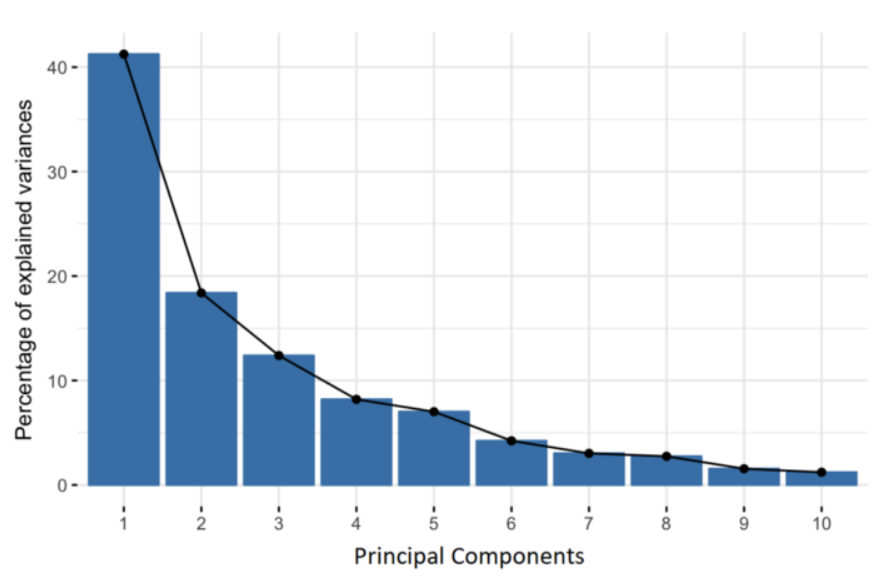
\includegraphics[width=100mm,scale=1]{Images/A5_img1.PNG}}
Organizing information in principal components this way, will allow you to reduce dimensionality without losing much information, and this by discarding the components with low information and considering the remaining components as your new variables.

An important thing to realize here is that, the principal components are less interpretable and don’t have any real meaning since they are constructed as linear combinations of the initial variables.

Geometrically speaking, principal components represent the directions of the data that explain a maximal amount of variance, that is to say, the lines that capture most information of the data. The relationship between variance and information here, is that, the larger the variance carried by a line, the larger the dispersion of the data points along it, and the larger the dispersion along a line, the more the information it has. To put all this simply, just think of principal components as new axes that provide the best angle to see and evaluate the data, so that the differences between the observations are better visible. \\[0.2 cm]
\textcolor{purple}{\centerline{\underline{{ Step 4: Feature Vector }}}}\\[0.2 cm]
Computing the eigenvectors and ordering them by their eigenvalues in descending order allow us to find the principal components in order of significance. In this step, what we do is, to choose whether to keep all these components or discard those of lesser significance (of low eigenvalues), and form with the remaining ones a matrix of vectors that we call Feature vector.

So, the feature vector is simply a matrix that has as columns the eigenvectors of the components that we decide to keep. This makes it the first step towards dimensionality reduction, because if we choose to keep only p eigenvectors (components) out of n, the final data set will have only p dimensions.
Thus, it’s up to you to choose whether to keep all the components or discard the ones of lesser significance, depending on what you are looking for. Because if you just want to describe your data in terms of new variables (principal components) that are uncorrelated without seeking to reduce dimensionality, leaving out lesser significant components is not needed.\\[0.2 cm]
\textcolor{purple}{\centerline{\underline{{Step 5: Recast the Data Along the Principal Components Axes }}}}\\[0.2 cm]
In the previous steps, apart from standardization, you do not make any changes on the data, you just select the principal components and form the feature vector, but the input data set remains always in terms of the original axes (i.e, in terms of the initial variables).

In this step, which is the last one, the aim is to use the feature vector formed using the eigenvectors of the covariance matrix, to reorient the data from the original axes to the ones represented by the principal components (hence the name Principal Components Analysis). This can be done by multiplying the transpose of the original data set by the transpose of the feature vector.\\[0.2 cm]
\centerline{$FinalDataSet$ = $FeatureVector^T$ * $StandardizedOriginalDataset^T$}